
\sect{Youtube Premiere}

Eine Youtube Premiere kann man einfach über die Webseite starten.
OBS oder OBS Studio werden hier nicht benötigt. \\


\newpage

\sub{Upload des Videos}

{\vspace{0.2cm}}
\begin{center}
  \textbf{Hierfür klickt hierfür auf \quote{Erstellen} rechts oben.} \\
  {\vspace{0.3cm}}
  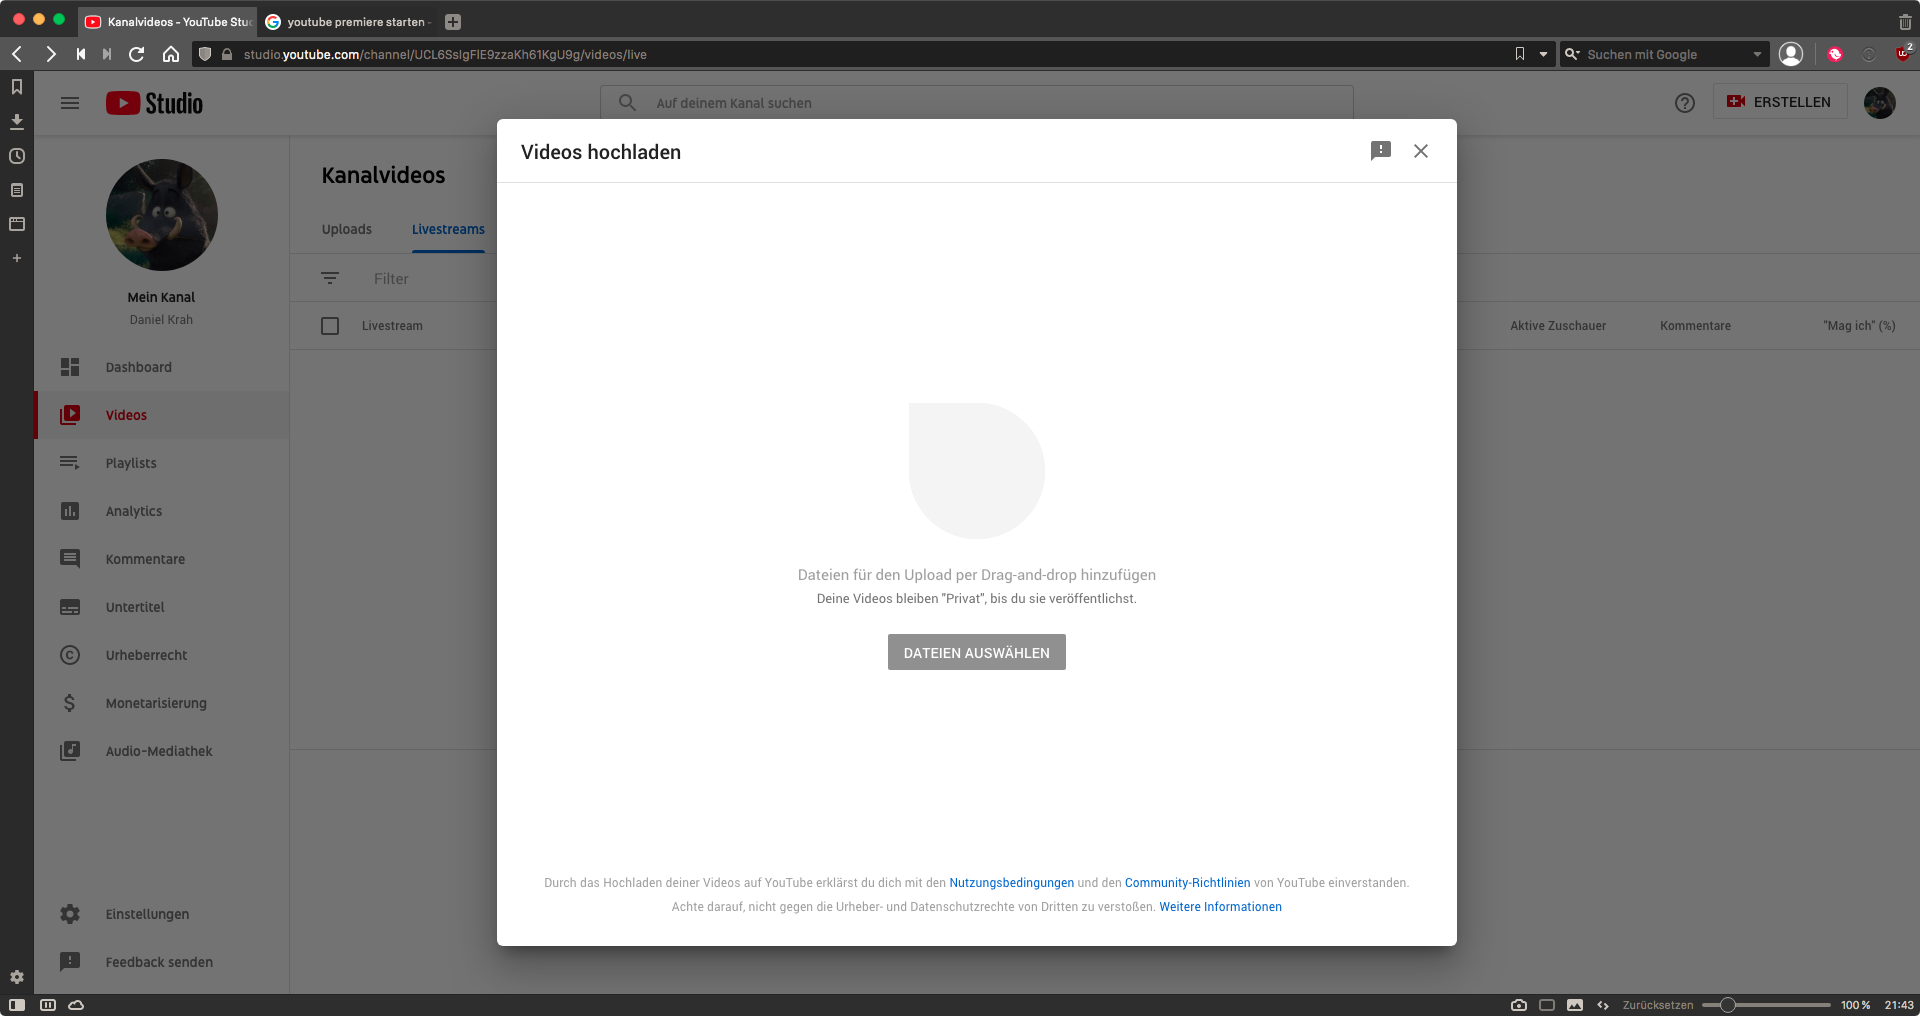
\includegraphics[width=\textwidth]{./pictures/premiere1.png}
\end{center}



% {\vspace{-0.6cm}}
\begin{center}
  \textbf{Hier ist es wichtig die Zielgruppeneinstellung zu setzen.} \\
  {\vspace{0.3cm}}
  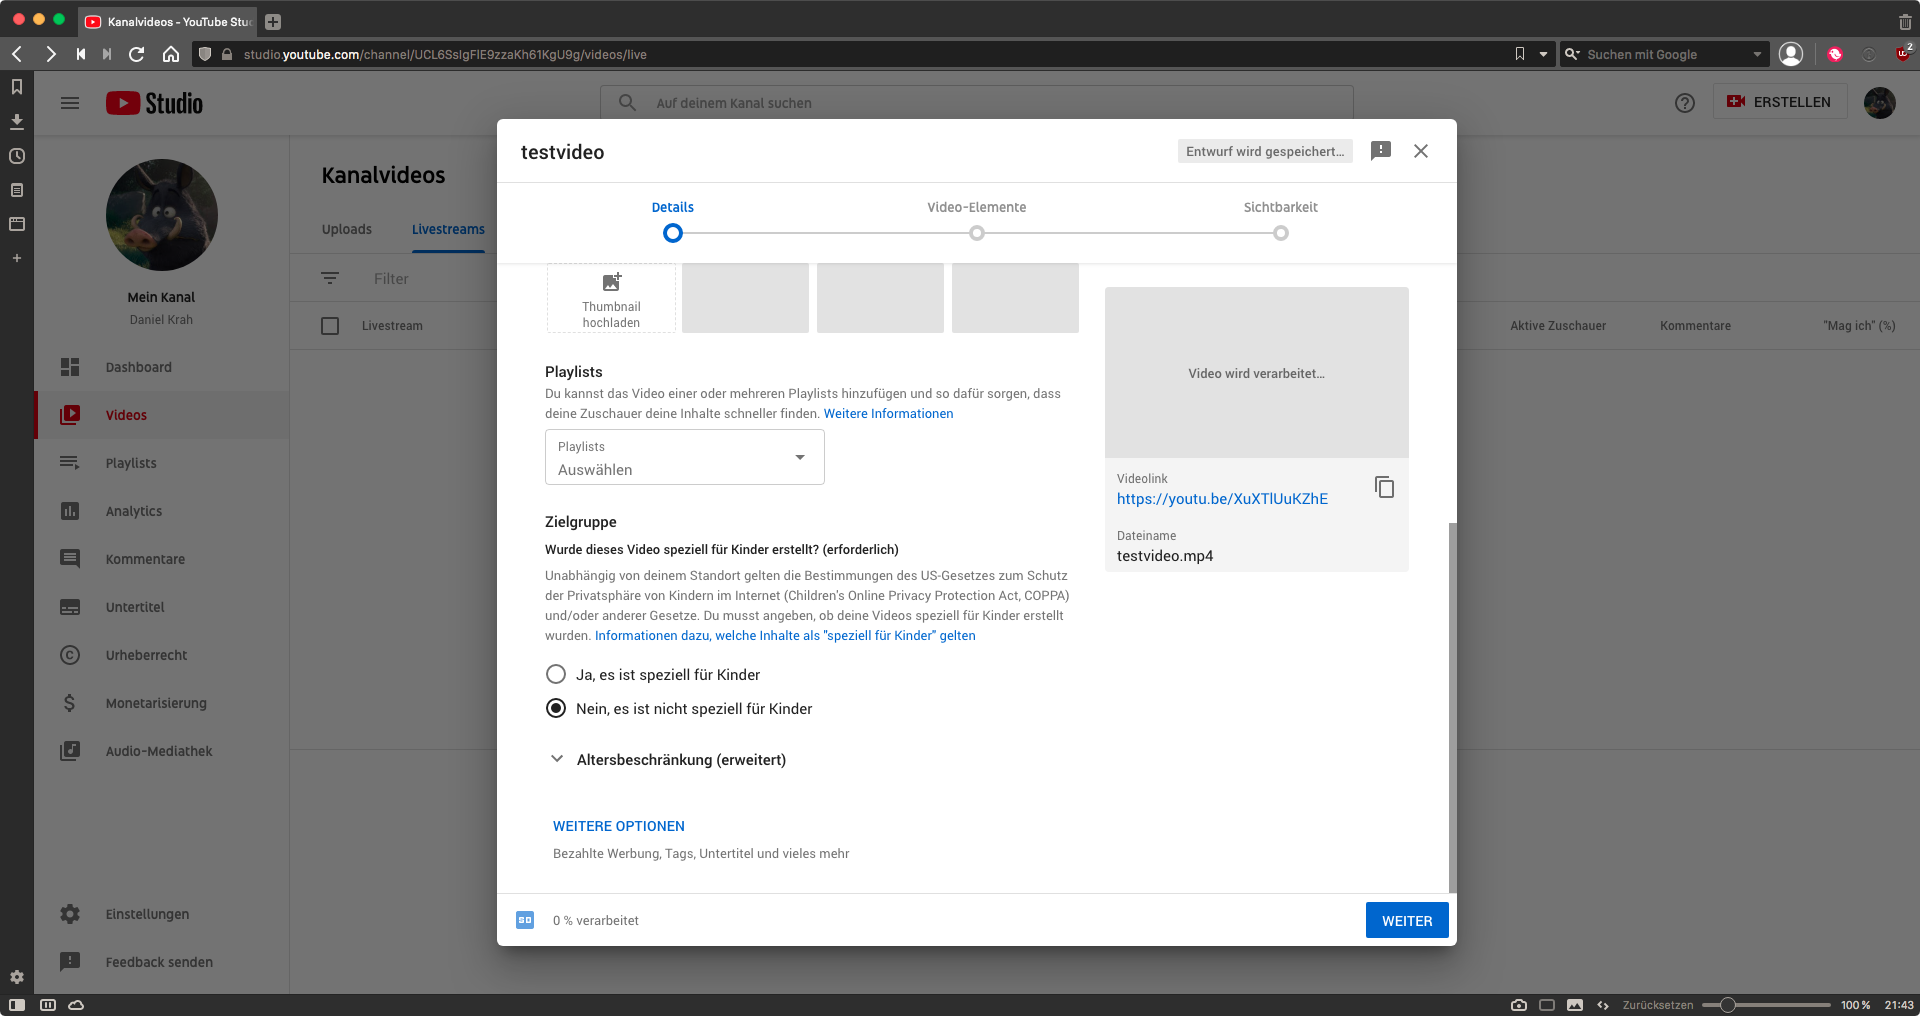
\includegraphics[width=\textwidth]{./pictures/premiere2.png}
\end{center}

\newpage
% {\vspace{-0.6cm}}
\begin{center}
  \textbf{Im nächsten Schritt kann man Infokarten oder einen extra Abspann hinzufügen.} \\
  {\vspace{0.3cm}}
  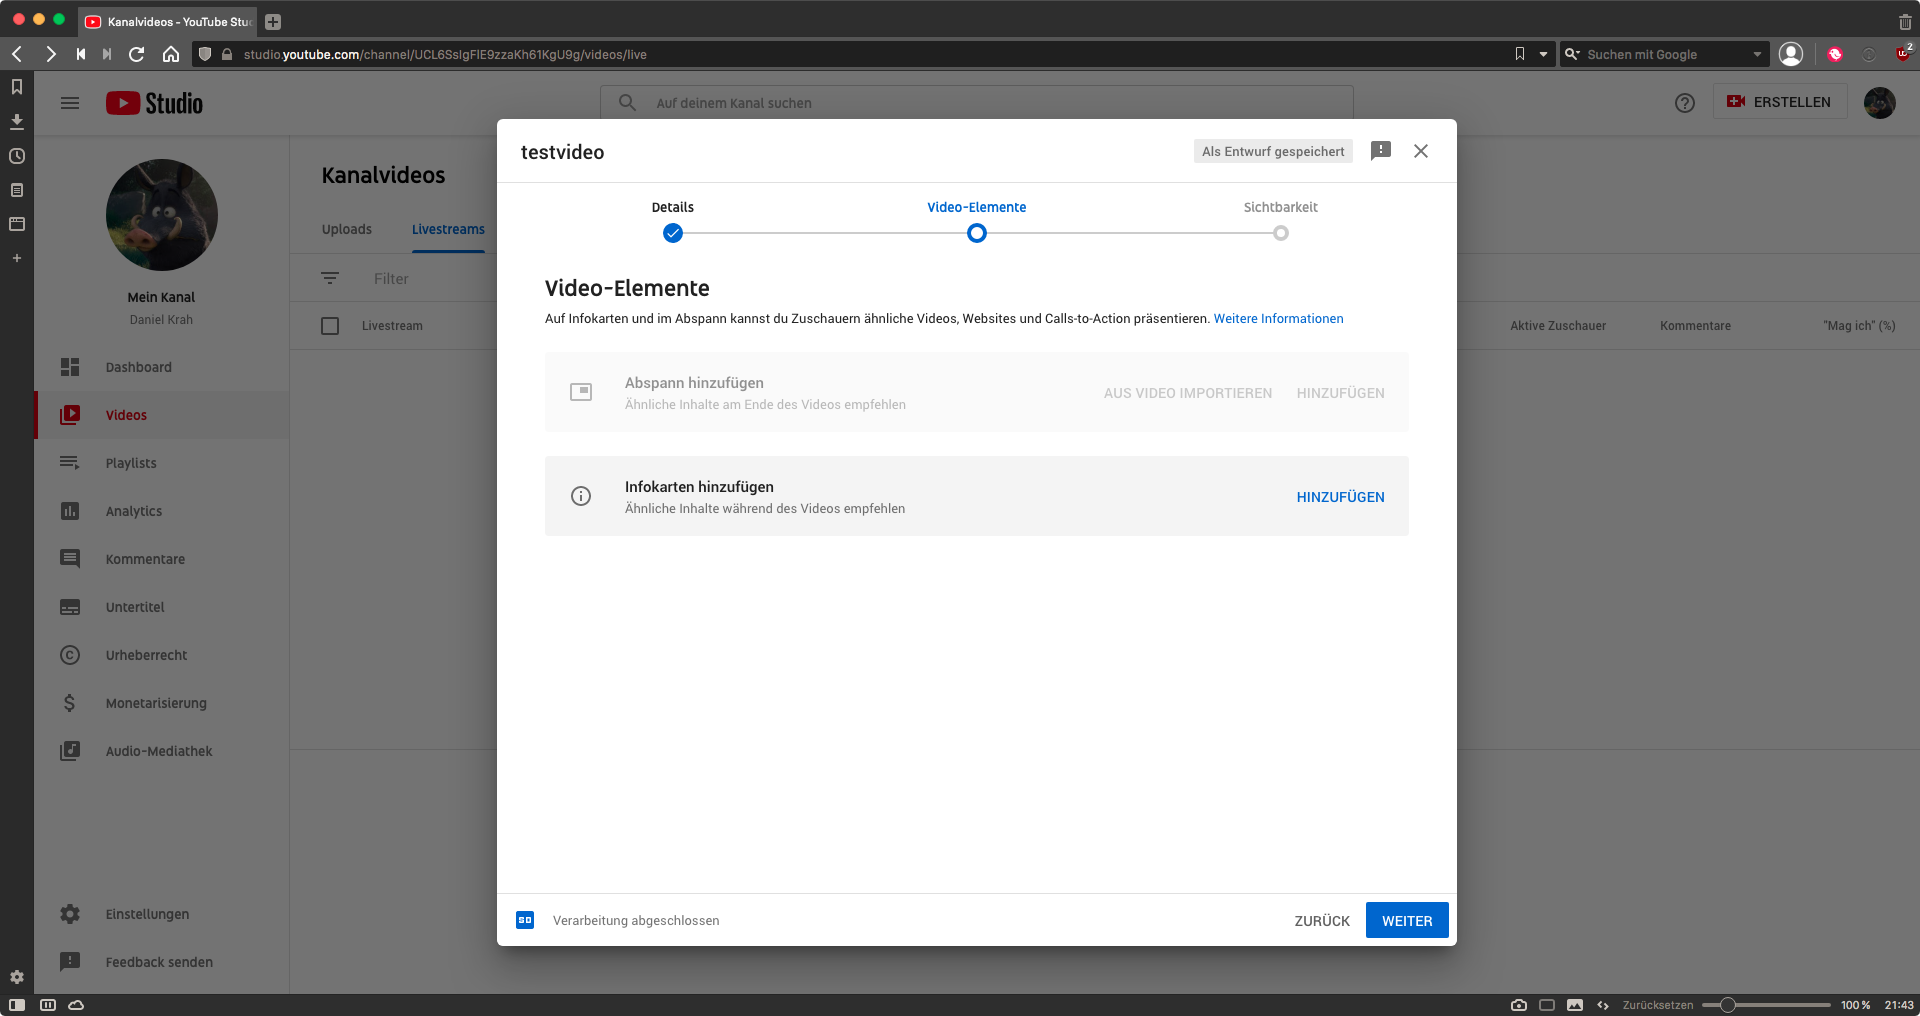
\includegraphics[width=\textwidth]{./pictures/premiere3.png}
\end{center}


% {\vspace{-0.6cm}}
\begin{center}
  \textbf{Zu guter Letzt legt man das Veröffentlichungsdatum und Uhrzeit fest. } \\
  \textbf{Wichtig ist hierbei das Häkchen bei Premiere zu setzen} \\
  {\vspace{0.3cm}}
  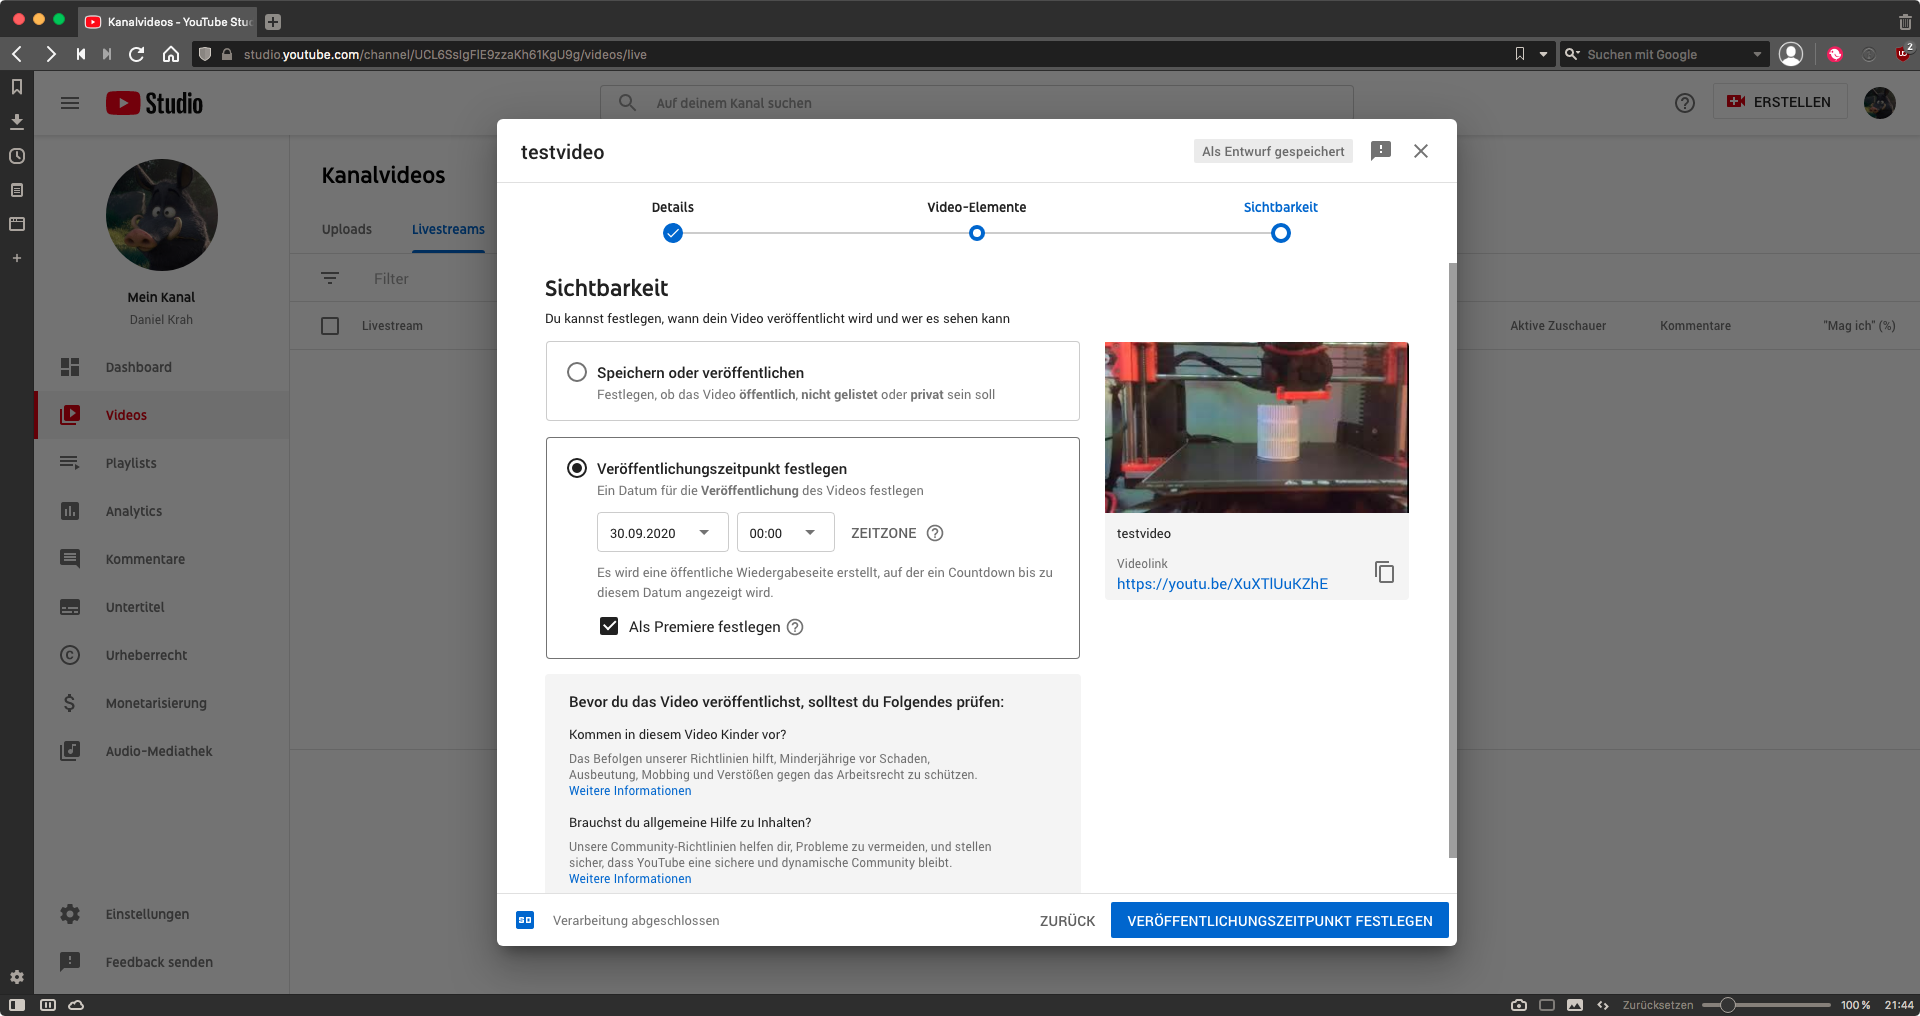
\includegraphics[width=\textwidth]{./pictures/premiere4.png}
\end{center}

\newpage
% {\vspace{-0.6cm}}
\begin{center}
  \textbf{Wenn alles erledigt ist bekommt man noch mal eine Übersicht, sowie vorbereitete Links für Social Media oder die eigene Webseite zum Einbinden.} \\
  {\vspace{0.3cm}}
  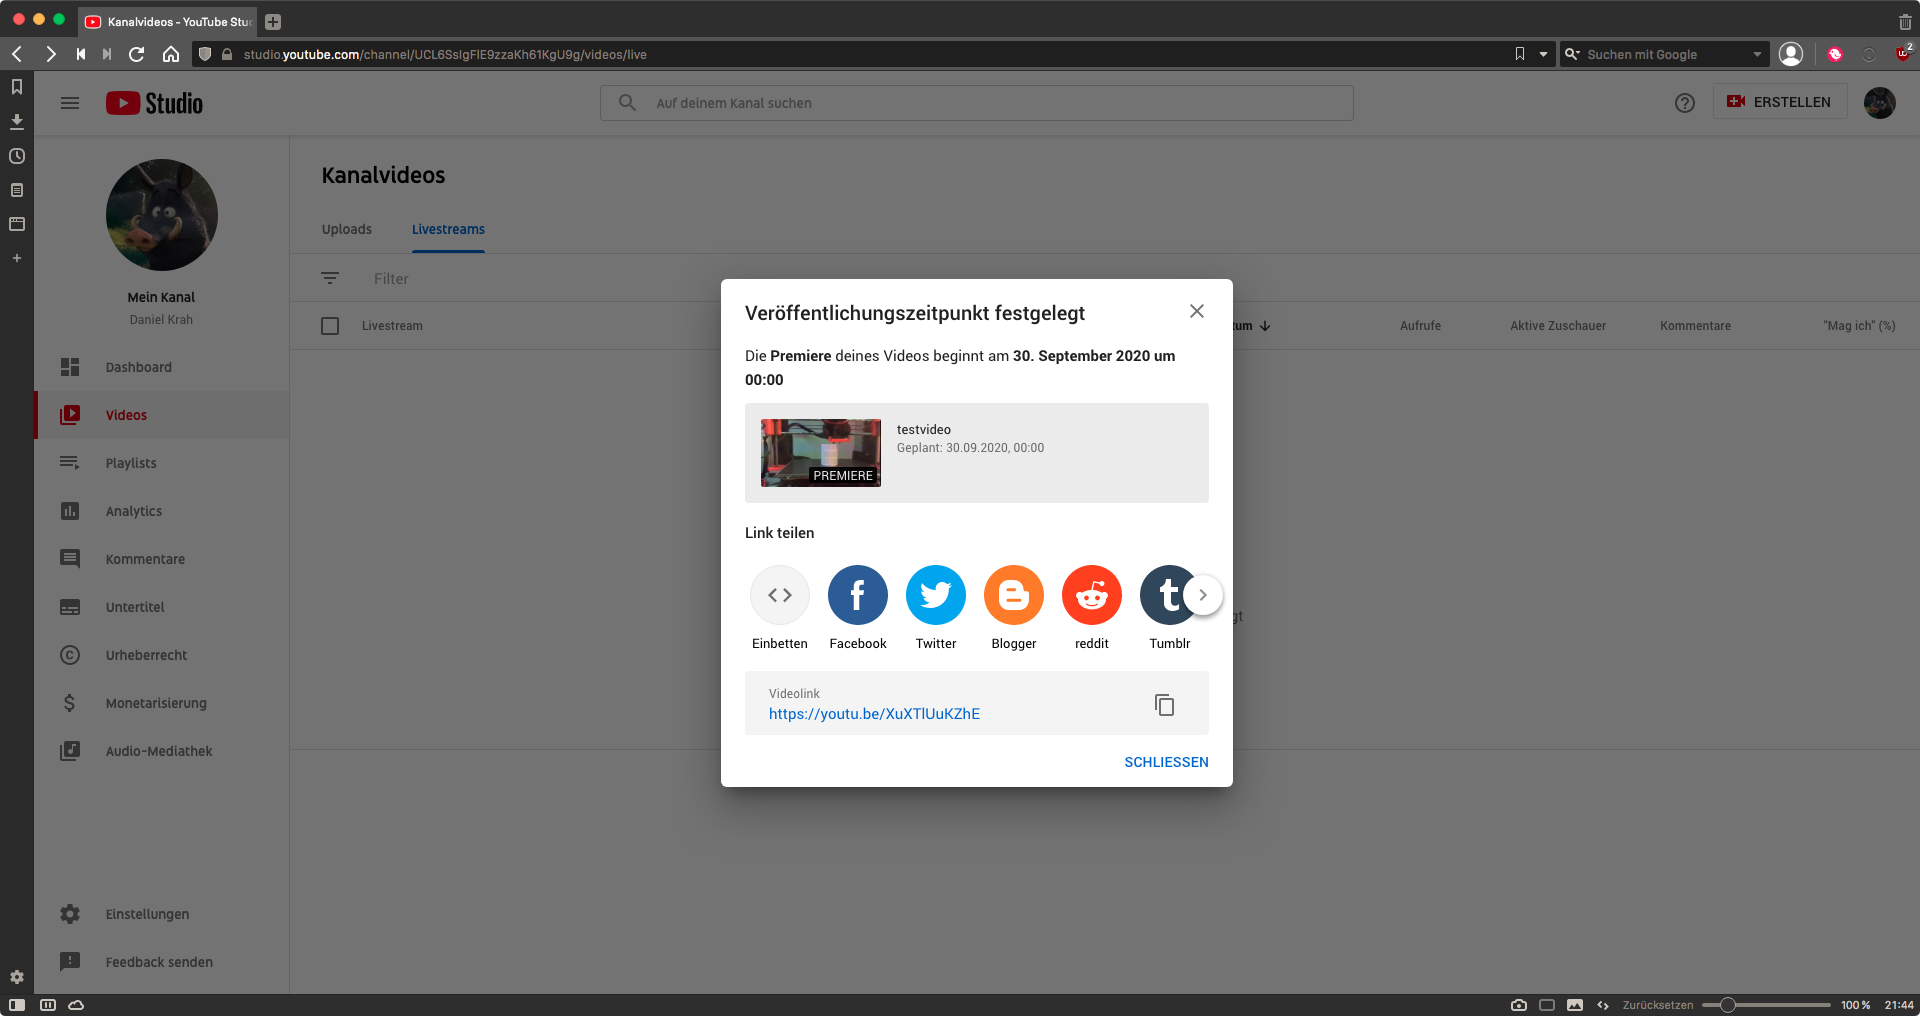
\includegraphics[width=\textwidth]{./pictures/premiere5.png}
\end{center}

% {\vspace{-0.6cm}}
\begin{center}
  \textbf{Hier als Beispiel der Quelltext zum einbinden in die Eigene Webseite.} \\
  {\vspace{0.3cm}}
  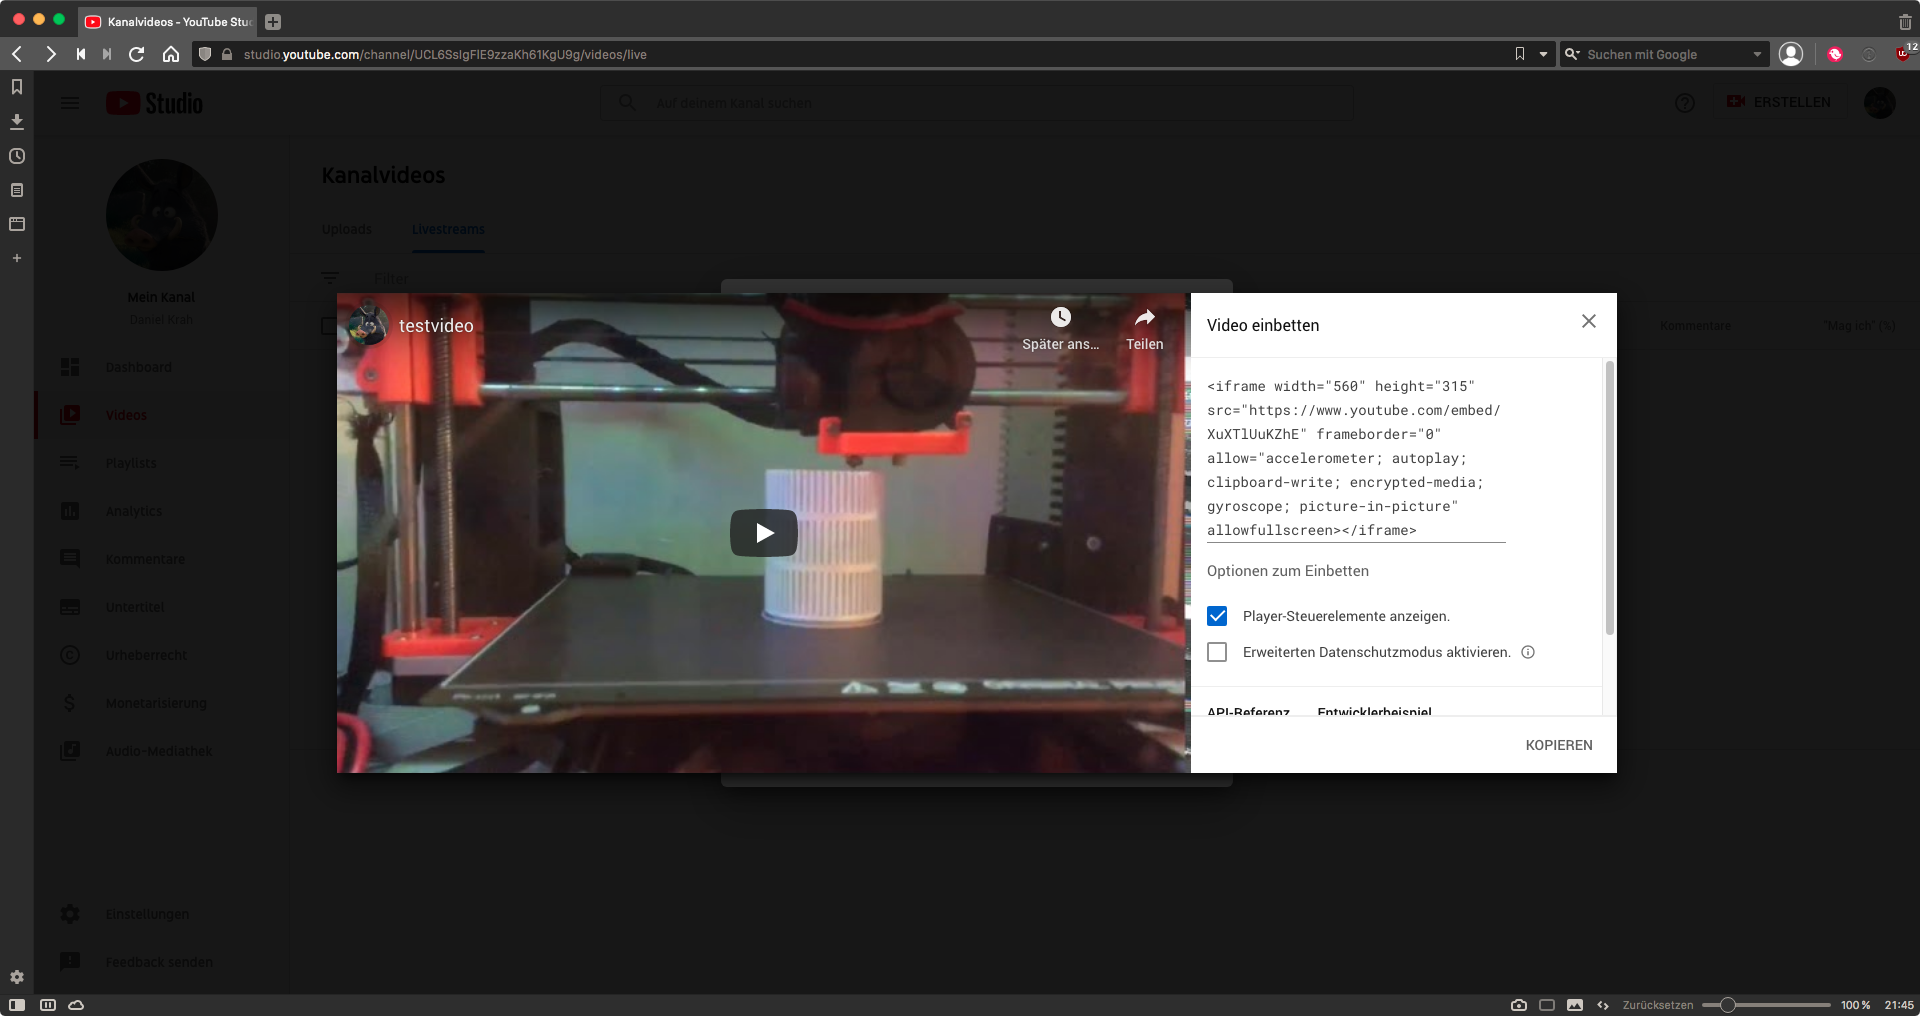
\includegraphics[width=\textwidth]{./pictures/premiere6.png}
\end{center}

\newpage
\sub{Erweiterte Einstellungen}
% {\vspace{-2.6cm}}
\begin{center}
  \textbf{Als nächstes kann man weitere Einstellungen über das Youtube Studio vornehmen} \\
  \textbf{Die Premiere befindet sich dann unter dem Livestreams-Tab} \\
  {\vspace{0.3cm}}
  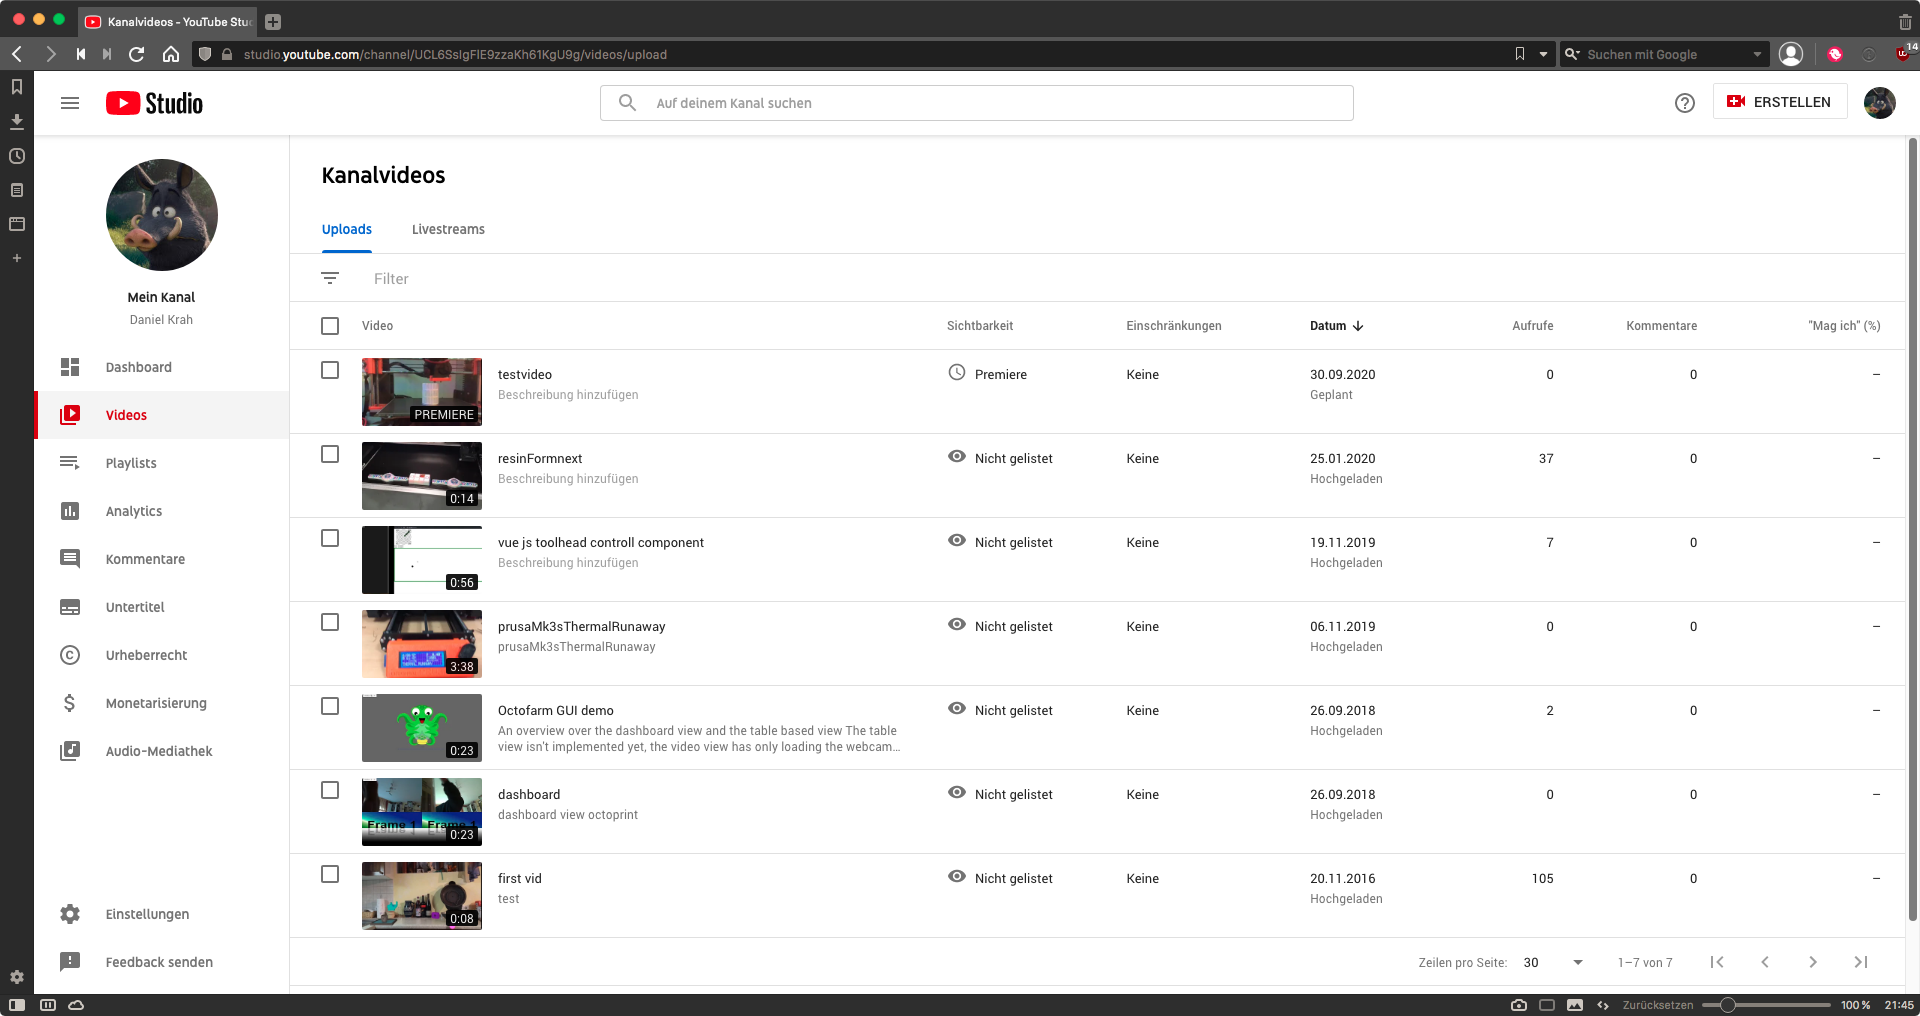
\includegraphics[width=\textwidth]{./pictures/premiere7.png}
\end{center}

% {\vspace{-0.6cm}}
\begin{center}
  \textbf{Unter \quote{Weitere Optionen sind die unten abgebildeten Einstellungen zu setzen.}} \\
  \textbf{Zusätzlich kann man den Livechat nach der Premiere ungelöscht lassen.}
  % {\vspace{0.3cm}}
  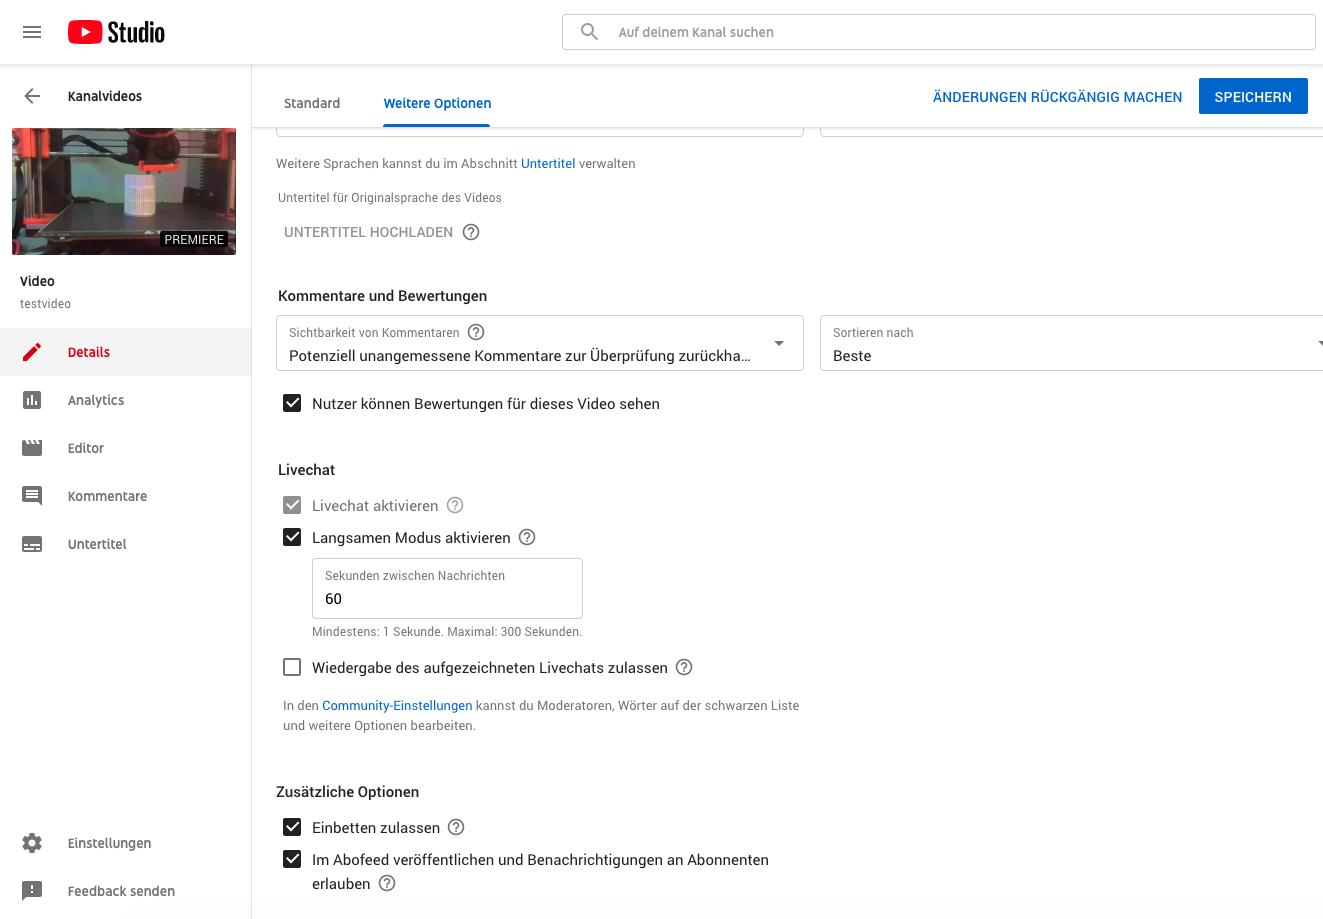
\includegraphics[width=0.8\textwidth]{./pictures/premiere8.png}
\end{center}

\newpage
\sub{Community Einstellungen}
% {\vspace{-0.6cm}}
\begin{center}
  \textbf{Wenn man auf Community-Einstellungen geklickt hat kann man nun die Schimpfwort-Filter anstellen} \\
  {\vspace{0.3cm}}
  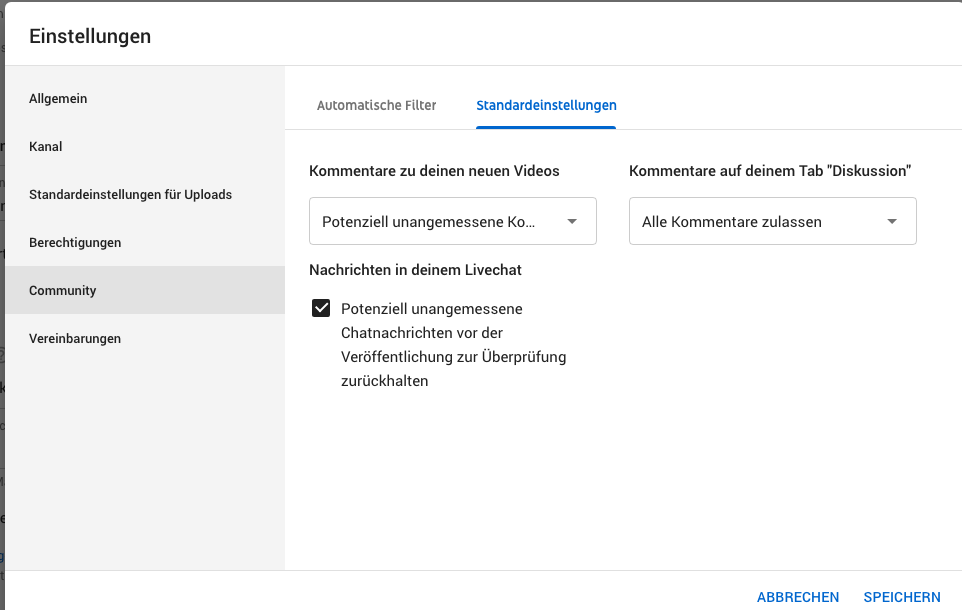
\includegraphics[width=\textwidth]{./pictures/premiere10.png}
\end{center}

% {\vspace{-0.6cm}}
\begin{center}
  \textbf{Im Tab \quote{Automatische Filter} kann man Moderatoren hinzufügen} \\
  {\vspace{0.3cm}}
  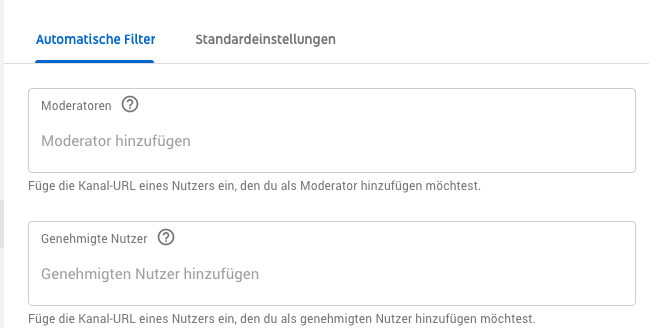
\includegraphics[width=\textwidth]{./pictures/premiere9.png}
\end{center}
\newpage


% {\vspace{-0.6cm}}
\begin{center}
  \textbf{Sowie Bestimmte selbst gewählte Wörter Sperren} \\
  {\vspace{0.3cm}}
  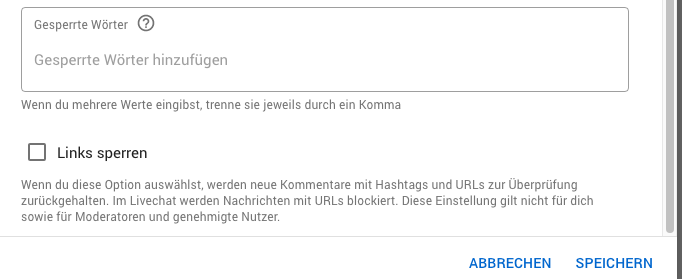
\includegraphics[width=\textwidth]{./pictures/premiere11.png}
  \textbf{Das verbieten von Links ist Sinnvoll. Moderatoren können trotzdem Links im Chat posten} \\
\end{center}


Die Premiere verhält sich genau wie ein Livestream. Für den Chat kann man dann einfach den Webbrowser benutzen und benötigt kein Streamlabs OBS/OBS.

\sect{Fazit}

Die Premiere inklusive der Einbindung auf die eigene Webseite ist die beste Möglichkeit das Festival umzusetzen. \\
Durch die likes/dislikes bekommt man auch einen guten Überblick wie gut der jeweilige Film ankam.
